\section{Homework 2: Nonparametric Statistics}

\subsection{Problem 1}

Given a random sample $X_1, \ldots, X_n$, show that the maximization of the empirical likelihood gives the empirical distribution function
\[
\hat{F}(x) = \frac{1}{n} \sum_{i=1}^{n} I(X_i \leq x).
\]

\subsubsection*{(a) Unique values (no tie)}

\textbf{解答：}

目标：maximize $L(F) = \prod_{i=1}^{n} F(x_i) = \prod_{i=1}^{n} [F(X_i) - F(X_{i-})]$.

对于 $X_1, \ldots, X_n$, $X_i \neq X_j$ ($i \neq j$), maximize $L(F) \Leftarrow$ maximize $\prod q_i$, where $\sum q_i = 1$.

而有 $\sqrt[n]{\prod q_i} \leq \frac{\sum q_i}{n}$, ``$=$'' $\Leftrightarrow$ $q_1 = \cdots = q_n = \frac{\sum q_i}{n} = \frac{1}{n}$.

即 $\hat{F}(x) = \frac{1}{n} \sum_{i=1}^{n} I(X_i \leq x)$.

\subsubsection*{(b) General case with ties}

\textbf{解答：}

maximize $L(F) \Leftarrow$ maximize $\prod_{i=1}^{K} q_i^{n_i}$, where $\sum_{i=1}^{K} n_i = n$ \& $\sum q_i = 1$.

即求 $\log \prod q_i^{n_i} = \sum n_i \log q_i$ 的最大值点.

可用 Lagrange 乘因子法, 令 $G = \sum n_i \log q_i - \lambda (\sum q_i - 1)$.

\[
\frac{\partial G}{\partial q_i} = 0 = \frac{n_i}{q_i} - \lambda \implies q_i = \frac{n_i}{\lambda}
\]

对 $q_i$ 求和有 $\sum q_i = \frac{\sum n_i}{\lambda} = \frac{n}{\lambda} = 1 \implies \lambda = n$.

即 $q_i = \frac{n_i}{n}$ ($i = 1, \ldots, K$). 可以验证对应为极大值点, 且即为最大值.

对应 $\hat{F}(x) = \frac{1}{n} \sum_{i=1}^{n} I(X_i \leq x)$, 因为在 $x_j$ 处 $F(x_j) - F(x_j-) = (\frac{1}{n}) \cdot n_j = q_j$.

\subsection{Problem 2}

Given a random sample $X_1, \ldots, X_n$, and the estimated density function with the Gaussian (standard normal) kernel $K(\cdot)$,
\[
\hat{f}(x) = \frac{1}{nh} \sum_{i=1}^{n} K\left(\frac{x - X_i}{h}\right),
\]
find $\int_{\mathbb{R}} x \hat{f}(x) dx$, $\int_{\mathbb{R}} x^2 \hat{f}(x) dx$, and $\int_{\mathbb{R}} x^2 \hat{f}(x) dx - \left(\int_{\mathbb{R}} x \hat{f}(x) dx\right)^2$. How would you interpret these results?

\textbf{解答：}

\begin{align*}
\int_{\mathbb{R}} x \hat{f}(x) dx &= \frac{1}{nh} \sum_{i=1}^{n} \int_{\mathbb{R}} x K\left(\frac{x - X_i}{h}\right) dx \\
&= \underset{u = \frac{x - X_i}{h},\, x = X_i + hu,\, du = hdx}{=} \frac{1}{n} \sum_{i=1}^{n} X_i \int_{\mathbb{R}} K(u) du + \frac{h}{n} \sum_{i=1}^{n} \int_{\mathbb{R}} u K(u) du \\
&= \frac{1}{n} \sum_{i=1}^{n} X_i = \bar{X}
\end{align*}

\begin{align*}
\int_{\mathbb{R}} x^2 \hat{f}(x) dx &= \frac{1}{nh} \sum_{i=1}^{n} \int_{\mathbb{R}} (X_i + hu)^2 K(u) du \\
&= \frac{1}{n} \sum X_i^2 + \frac{2h}{n} \sum_{i=1}^{n} X_i \int_{\mathbb{R}} u K(u) du + \frac{h^2}{n} \sum_{i=1}^{n} \int_{\mathbb{R}} u^2 K(u) du \\
&= \frac{1}{n} \sum X_i^2 + h^2
\end{align*}

将上两式代入得
\[
\int_{\mathbb{R}} x^2 \hat{f}(x) dx - \left(\int_{\mathbb{R}} x \hat{f}(x) dx\right)^2 = \frac{1}{n} \sum_{i=1}^{n} (X_i - \bar{X})^2 + h^2.
\]

\textbf{Interpret:} 用 Gaussian Kernel 估计密度函数, 二者一阶矩相同, 二阶矩增大了 $h^2$, 是因为光谱化导致矩增大. 当 $h \to 0$ 时有该方法的二阶矩 $\to$ 原二阶矩. 对均值是无偏估计.

\subsection{Problem 3}

Consider the data with an outlier (mentioned in the lecture notes):
\begin{itemize}
\item Group 1: 1 2 3 4 5 6 7 8 9 10
\item Group 2: 7 8 9 10 11 12 13 14 15 16 17 18 19 20 200
\end{itemize}
Select an appropriate nonparametric test, calculate the test statistic (show your steps), and compute the $p$-value using the normal asymptotic distribution.

\textbf{解答：}

使用 Wilcoxon 2-sample unpaired test. (在 R 中得到 $W = 8$, $p$-value $= 0.0002229$)

$H_0: \mu_1 = \mu_2$, $H_1: \mu_1 \neq \mu_2$, $\alpha = 0.05$, 拒绝原假设 $\mu_1 = \mu_2$.

\textbf{手算 Rank:}

\begin{center}
\begin{tabular}{c|ccccccccccccccccc}
Group 1 & 1 & 2 & 3 & 4 & 5 & 6 & 7.5 & 9.5 & 11.5 & 13.5 & & & & & & & \\
Group 2 & 7.5 & 9.5 & 11.5 & 13.5 & 15 & 16 & 17 & 18 & $\cdots$ & 25 & & & & & & & \\
\end{tabular}
\end{center}

样本量 $m = 10$, $n = 15$. $W = \text{Group 1 rank 的和}$, $W = 63$.

\[
E(W) = \frac{m(m+n+1)}{2} = \frac{10(10+15+1)}{2} = 130
\]

\[
\text{Var}(W) = \frac{mn(m+n+1)}{12} = \frac{10 \times 15 \times 26}{12} = 325
\]

因此由 Normal-asymptotic distribution,
\[
W^* = \frac{63 - 130}{\sqrt{325}} \approx -3.72
\]

\[
p = 2\Phi(-3.72) \approx 0.0003
\]

拒绝原假设.

\subsection{Problem 4}

Verify that Spearman's correlation coefficient is equivalent to Pearson's correlation coefficient when applied to rank statistics, assuming no ties in the data.

\textbf{解答：}

Spearman: $r_s = \frac{12 \sum_{i=1}^{n} \left[(R_i - \frac{n+1}{2})(S_i - \frac{n+1}{2})\right]}{n(n^2 - 1)}$

$R_i, S_i$ 为 Rank of $X_i, Y_i$.

Pearson: $r_p = \frac{\sum_{i=1}^{n} (X_i - \bar{X}_n)(Y_i - \bar{Y}_n)}{\sqrt{\frac{1}{n}\sum_{i=1}^{n}(X_i - \bar{X}_n)^2} \sqrt{\frac{1}{n}\sum_{i=1}^{n}(Y_i - \bar{Y}_n)^2}}$

在其取 $X_{(k)} = k$, $Y_{(k)} = k$.

有 $\bar{X}_n = \frac{1}{n} \sum_{k=1}^{n} k = \frac{n+1}{2}$.

\begin{align*}
\frac{1}{n} \sum(X_i - \bar{X})^2 &= \frac{1}{n} \sum_{k=1}^{n} \left(k - \frac{n+1}{2}\right)^2 = \frac{1}{n} \sum_{k=1}^{n} \left[k^2 - (n+1)k\right] + \frac{1}{n} \cdot \frac{n(n+1)^2}{4} \\
&= \frac{1}{n} \left(\frac{1}{6}n(n+1)(2n+1) - \frac{1}{2}n(n+1)^2\right) + \frac{1}{4}(n+1)^2 \\
&= (n+1) \cdot \frac{1}{12}(n-1) = \frac{n^2 - 1}{12}
\end{align*}

$Y_i$ 对应项同理, 整理即得 $r_s$.

另有 $\sum(R_i - \frac{n+1}{2})(S_i - \frac{n+1}{2}) = \sum R_i S_i - \frac{n+1}{2}(\sum R_i + \sum S_i) + \frac{n(n+1)^2}{4} = \sum R_i S_i - \frac{n(n+1)^2}{4}$.

令 $D_i = R_i - S_i$, 则 $\sum R_i S_i = \frac{1}{2}\left(\sum R_i^2 + \sum S_i^2 - \sum D_i^2\right) = \frac{n(n+1)(2n+1)}{6} - \frac{1}{2}\sum D_i^2$.

代入化简即得 $r_s = 1 - \frac{6\sum D_i^2}{n(n^2 - 1)}$.

\subsection{Problem 5}

A medical research team wants to analyze the agreement between two clinicians (Clinician A and Clinician B) in rating the severity of a disease on a scale of 1 to 10. Each clinician independently assigns severity scores to 5 patients. The ratings are, in the form of (Clinician A's Rating, Clinician B's Rating): $(3, 4)$, $(7, 6)$, $(5, 3)$, $(9, 8)$, $(6, 7)$. Calculate the Kendall's tau coefficient. Show your steps.

\textbf{解答：}

Kendall's tau coefficient.

$(3,4)$, $(7,6)$, $(5,3)$, $(9,8)$, $(6,7)$, 记为 $A, B, C, D, E$.

\begin{center}
\begin{tabular}{ll}
Concordant: $AB$, $AD$, $AE$, $BC$, $BD$, $CD$, $CE$, $DE$ & 8个 \\
Discordant: $AC$, $BE$ & 2个 \\
\end{tabular}
\end{center}

\[
\tau = \frac{1}{\binom{5}{2}}(8 - 2) = \frac{6}{10} = 0.6
\]

\subsection{Problem 6}

Consider the BMI and cholesterol data at the baseline in the Framingham data.

\subsubsection*{(a) \& (b)}

使用R语言绘制QQ Plot并观察数据分布是否符合正态。可以发现Cholesterol和BMI的原始数据点偏离理论正态直线，尤其右尾偏离明显，右侧呈现重尾。采用取对数的方式对数据进行处理，绘制QQ Plot对比可以看出，数据偏离正态幅度减小，不过仍然呈现重尾。

\begin{center}
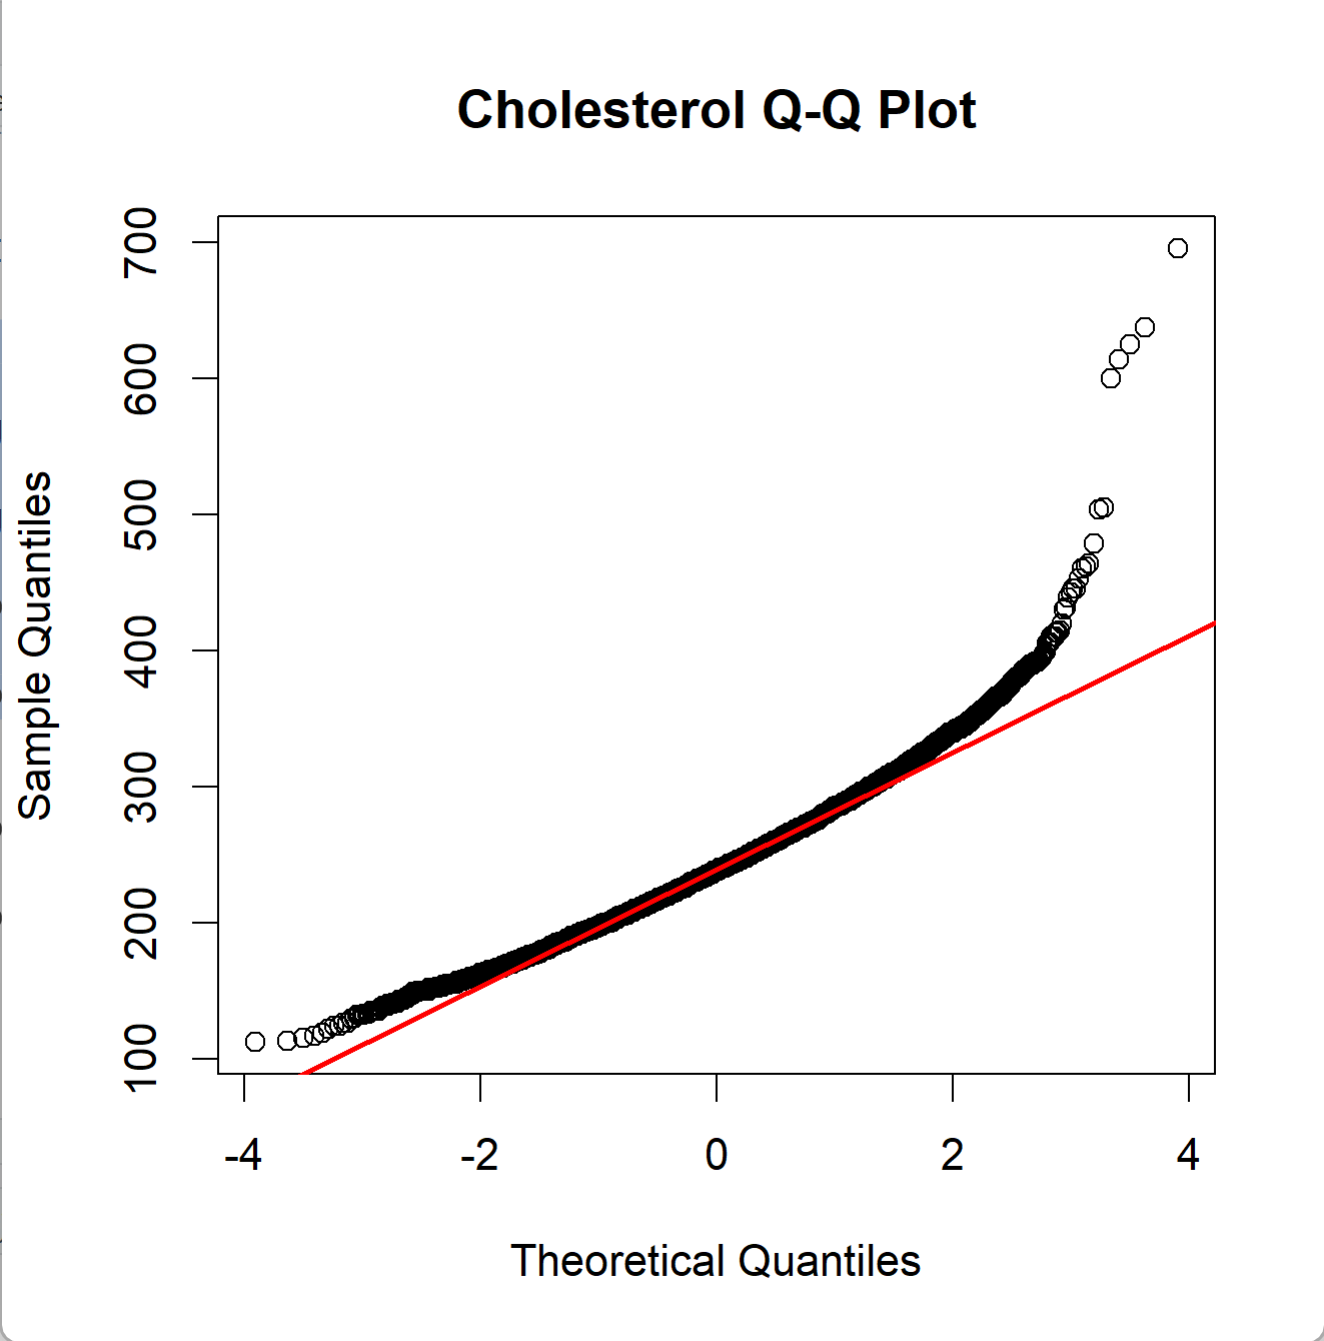
\includegraphics[width=0.8\textwidth]{figs/hw2_qq_cholesterol_original.png}
\end{center}

\begin{center}
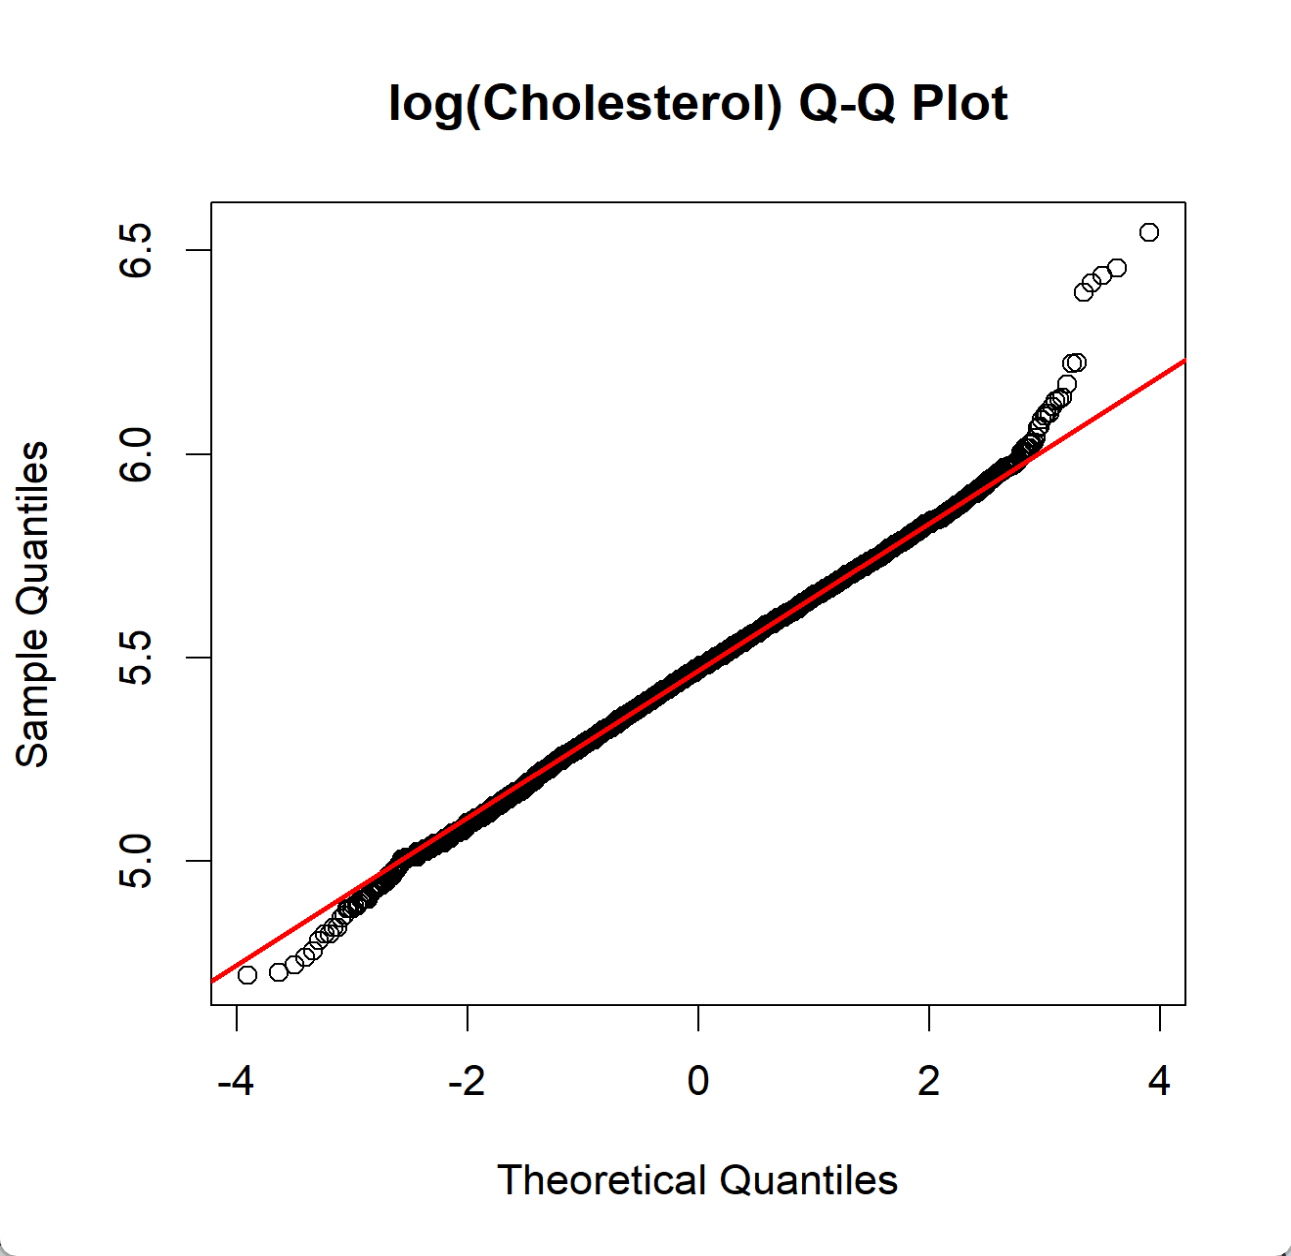
\includegraphics[width=0.8\textwidth]{figs/hw2_qq_cholesterol_log.png}
\end{center}

\begin{center}
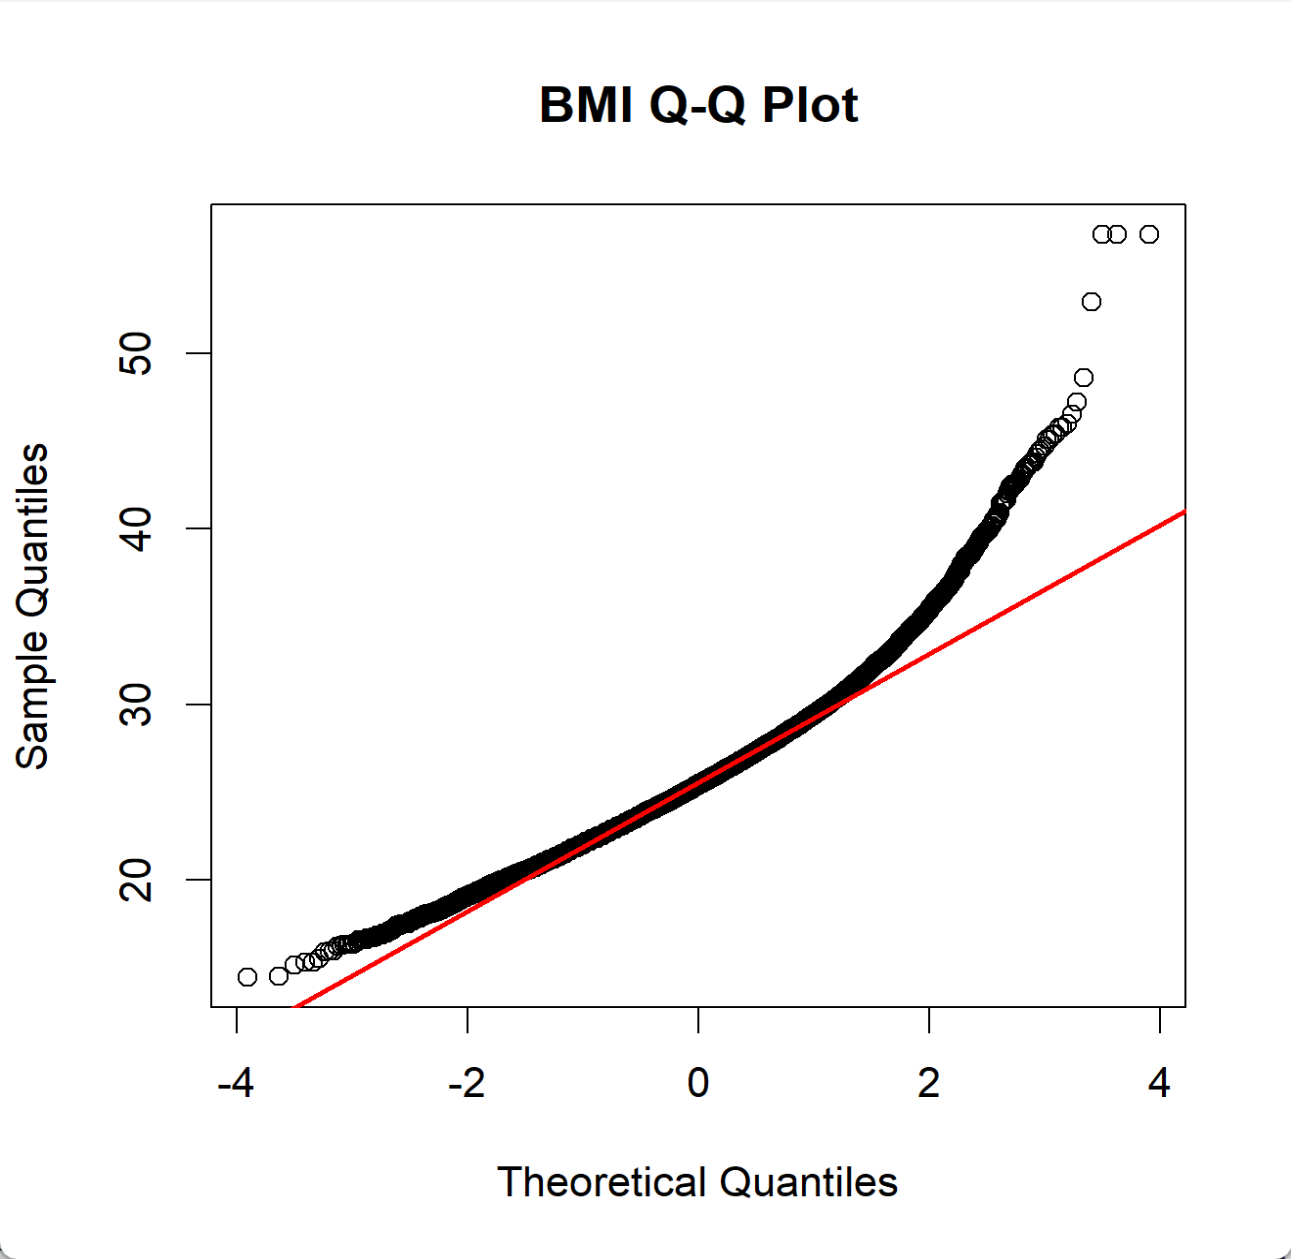
\includegraphics[width=0.8\textwidth]{figs/hw2_qq_bmi_original.png}
\end{center}

\begin{center}
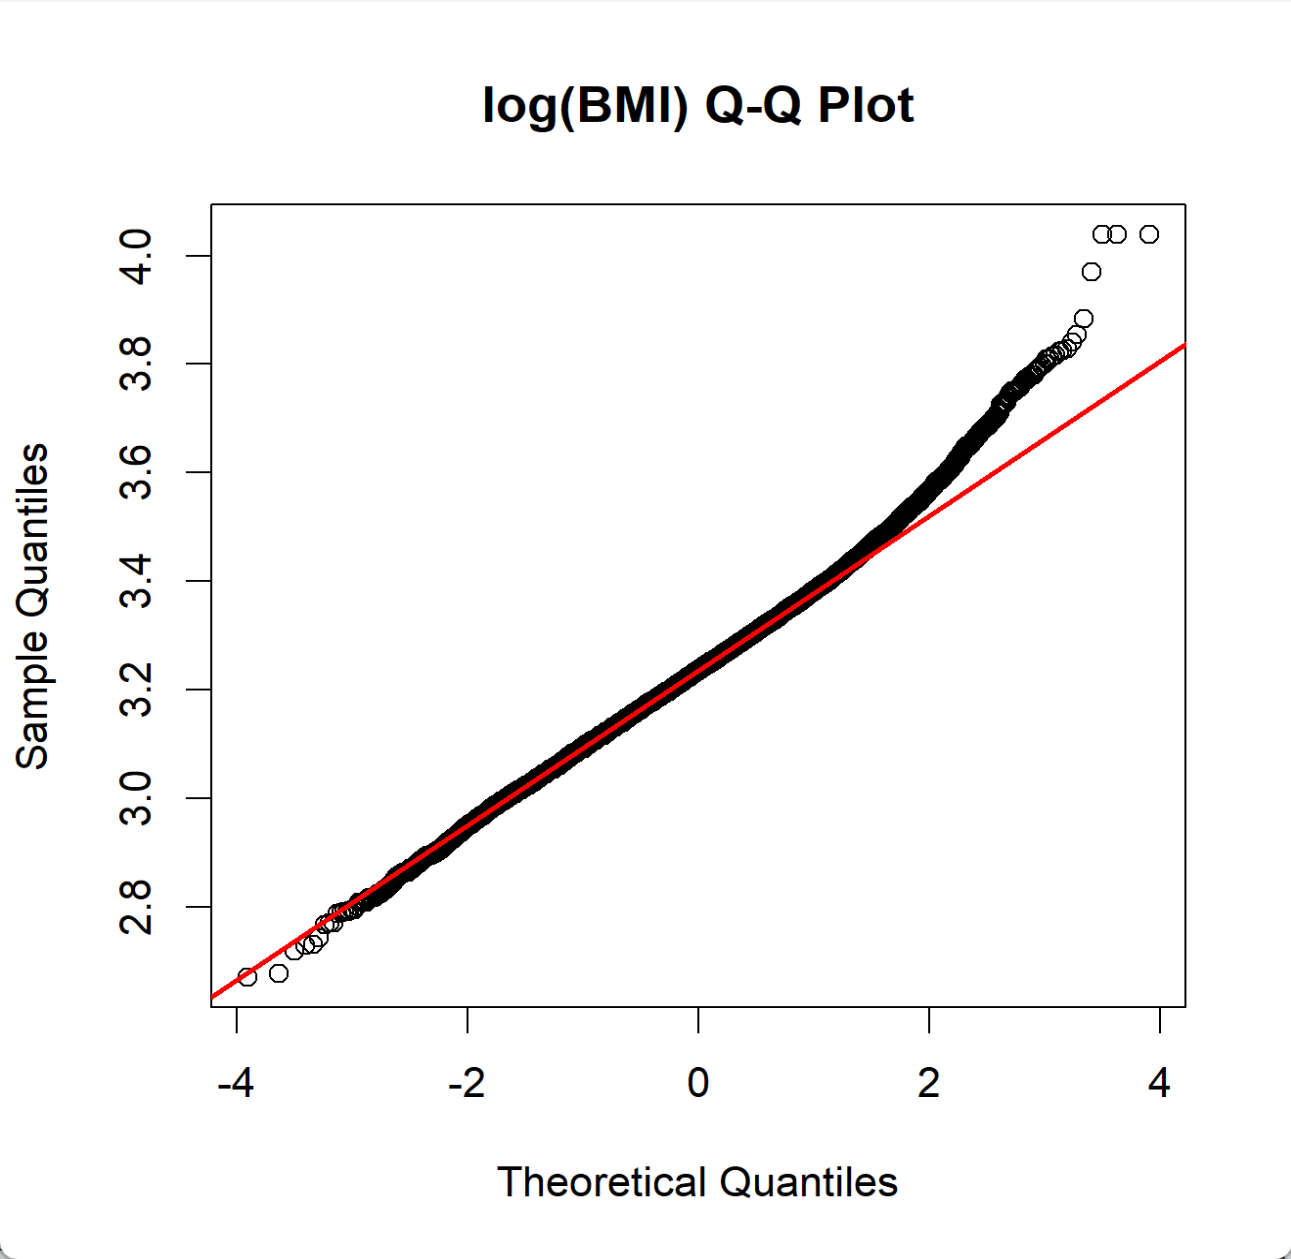
\includegraphics[width=0.8\textwidth]{figs/hw2_qq_bmi_log.png}
\end{center}

\subsubsection*{(c)}

考虑到样本量和可解释性，选用Pearson相关系数对未经变换的原数据进行计算。（在大样本情况下，Pearson 相关系数具有渐近正态性，因此对轻度偏离正态分布的样本具有稳健性，使用是合理的。）

计算得到 $\text{cor} = 0.0758$, 95\%置信区间为 $(0.0569, 0.0946)$, $p$-value $= 3.716 \times 10^{-15}$。有足够证据认为两者存在线性相关的关系，但相关系数数值较小（约 0.076），说明该线性关系在实际意义上比较弱。

此外可以计算 $\text{standard error} = \sqrt{\frac{1 - r^2}{n - 2}} = 0.00963$.

\subsubsection*{(d)}

图中直方图展示了通过 Bootstrap 方法（重复抽样1000次）得到的相关系数的经验分布，虚线表示原始样本计算得到的相关系数。可以看到，bootstrap 分布大致围绕该值对称分布。

\begin{center}
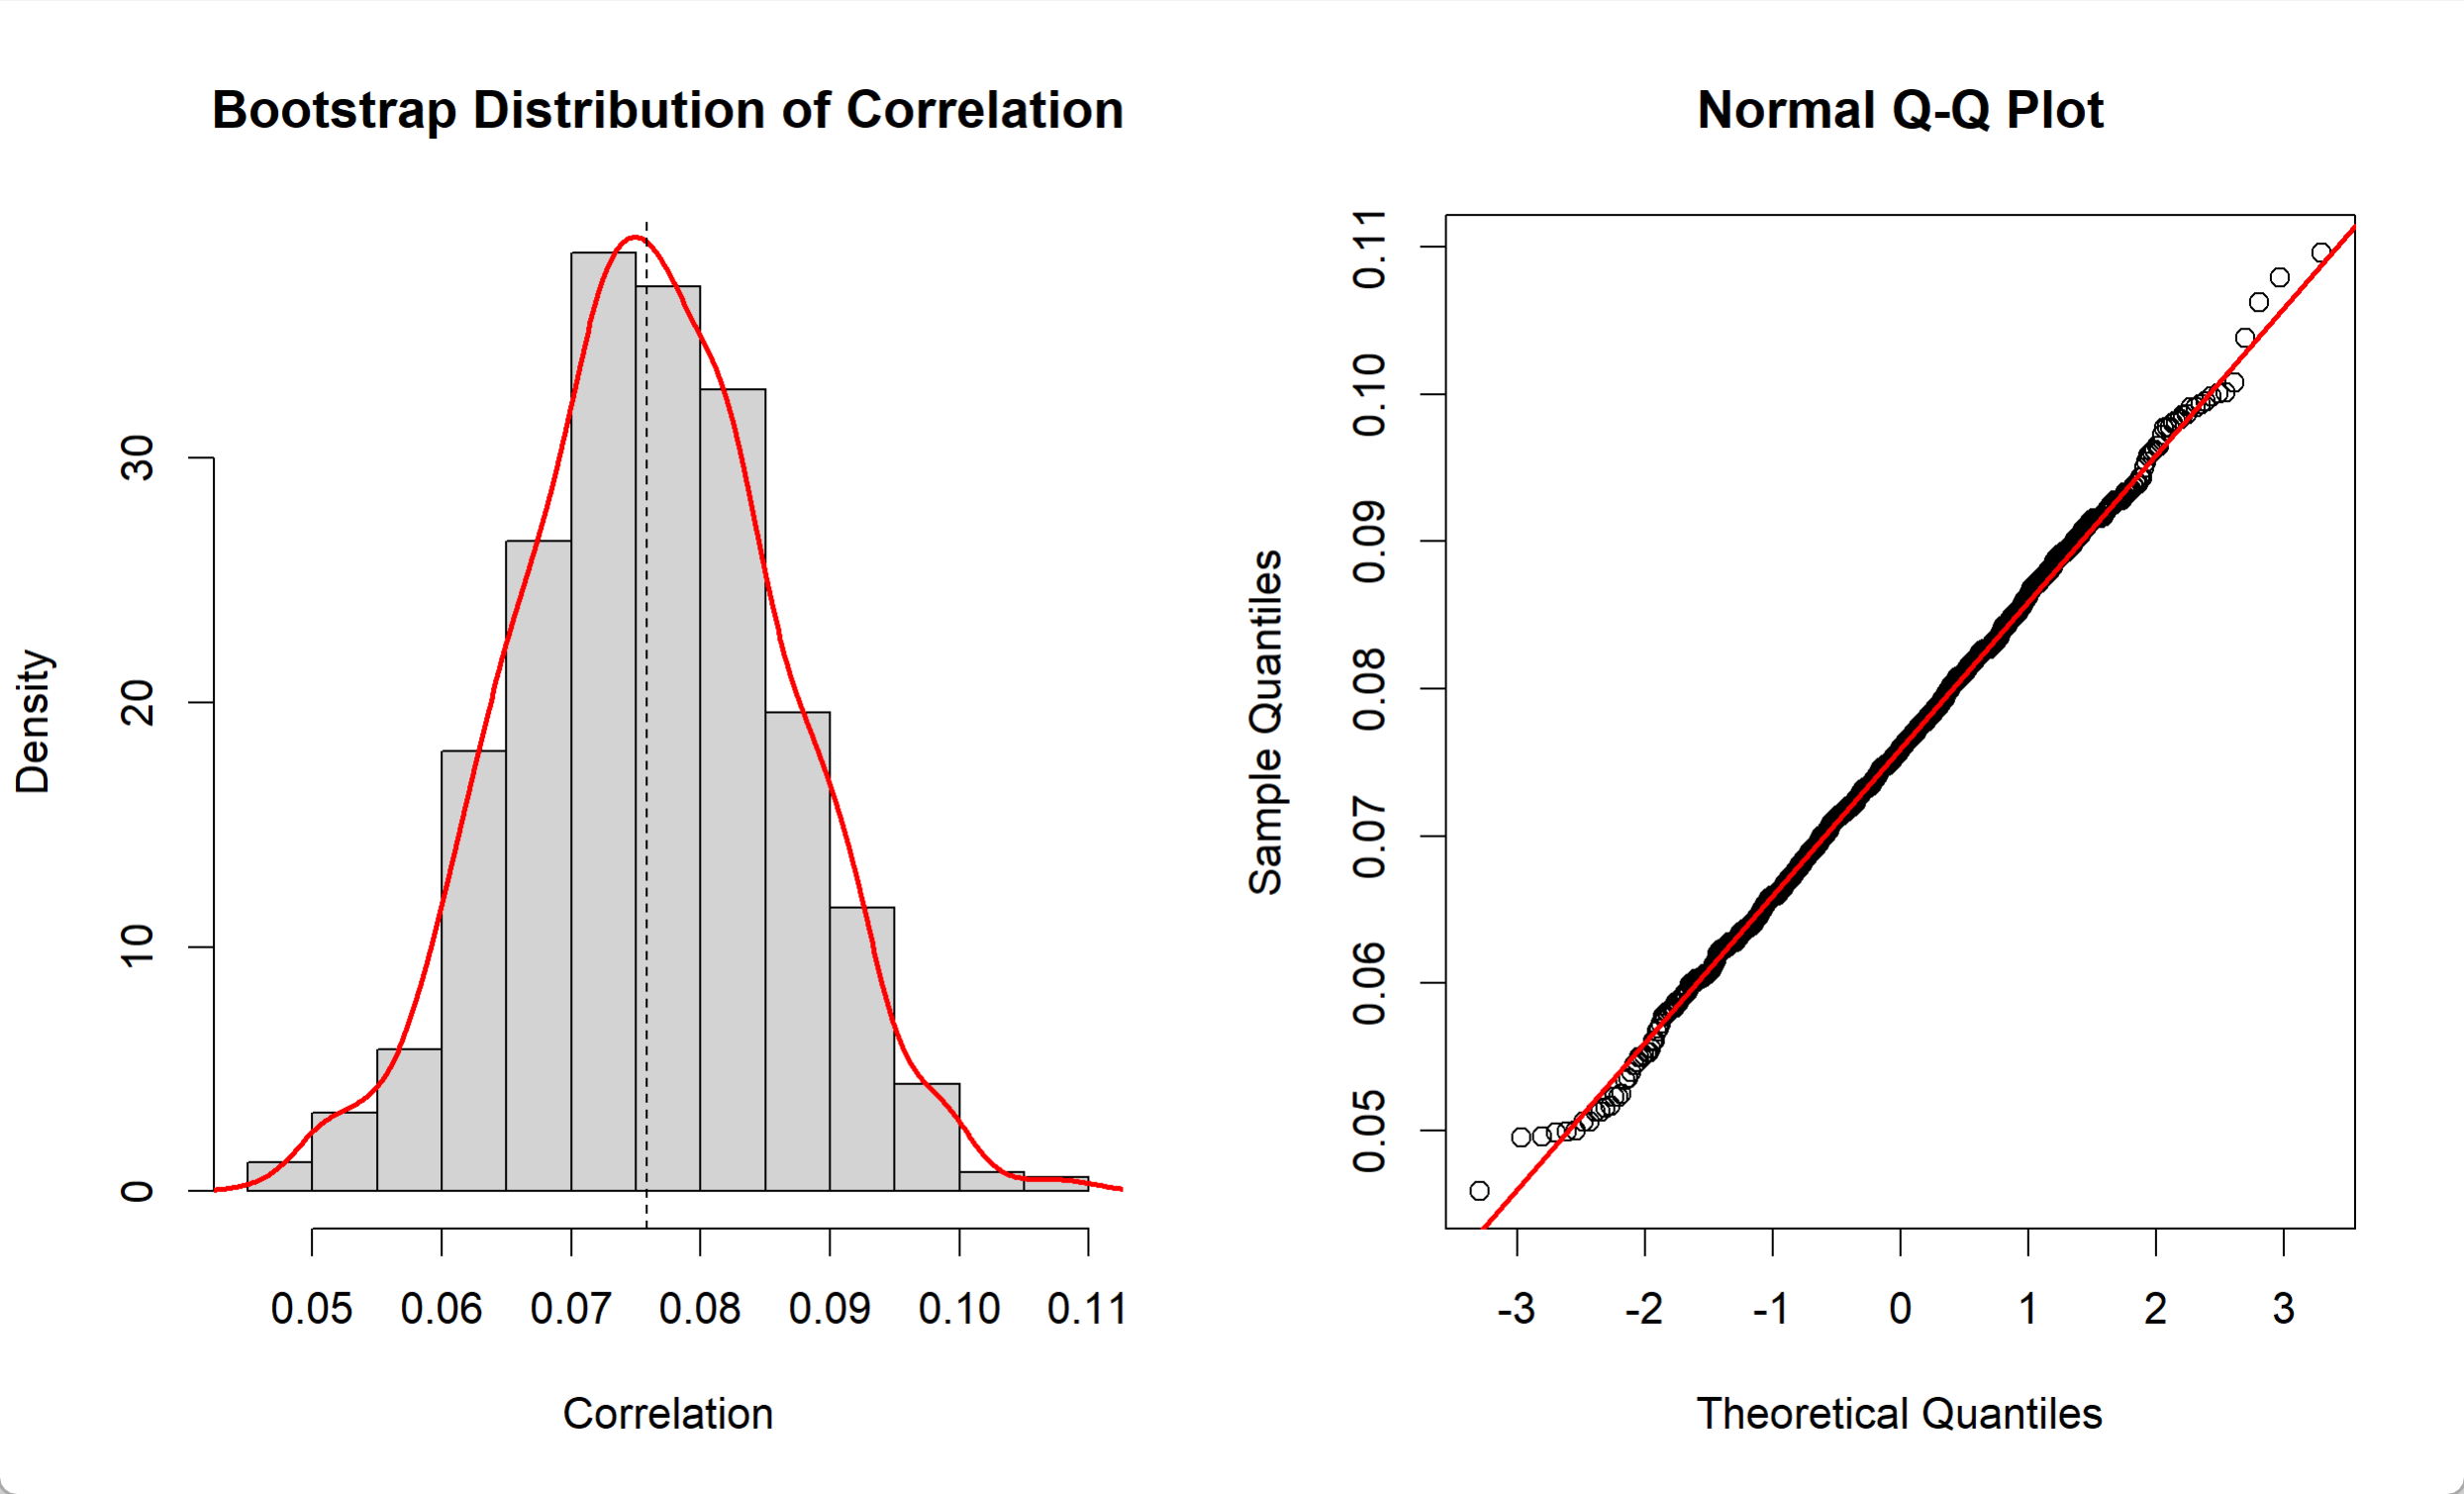
\includegraphics[width=0.8\textwidth]{figs/hw2_bootstrap_distribution.png}
\end{center}

通过直方图和QQ Plot可以看出Bootstrap得到的相关系数分布大致接近正态分布，这与 Pearson 相关系数在大样本下的渐近正态性是相符的。

Bootstrap方法计算的SE为0.0101，与理论计算得到的（0.00963）较为接近。具体地，相对偏差 $\frac{SE_{boot} - SE_{cal}}{SE_{cal}} \times 100\% = 4.88\%$，二者一致性较高。

\textbf{注：}

(1) 本题中对于缺失数据我们采用了删除的处理方式，仅保留BMI和TOTCHOL均有数据的样本（10726个）进行所有小问的分析，保证各问使用的数据一致。

(2) 本题所用代码见下：

\begin{lstlisting}[language=R]
# 6 a&b
df_clean <- df[complete.cases(df[, c("BMI", "TOTCHOL")]), ]
bmi <- df_clean$BMI
totchol <- df_clean$TOTCHOL

qqnorm(bmi, main = "BMI Q-Q Plot")
qqline(bmi, col = "red", lwd = 2)

bmilog <- log(bmi)
qqnorm(bmilog, main = "log(BMI) Q-Q Plot")
qqline(bmilog, col = "red", lwd = 2)

qqnorm(totchol, main = "Cholesterol Q-Q Plot")
qqline(totchol, col = "red", lwd = 2)

totchollog <- log(totchol)
qqnorm(totchollog, main = "log(Cholesterol) Q-Q Plot")
qqline(totchollog, col = "red", lwd = 2)

# 6 c
cor.test(bmi, totchol, method = "pearson")

# 6 d
# bootstrap
B <- 1000
n <- nrow(df_clean)
boot_cor <- numeric(B)
set.seed(100)

for (i in 1:B) {
  idx <- sample(1:n, size = n, replace = TRUE)
  boot_sample <- df_clean[idx, ]
  boot_cor[i] <- cor(boot_sample$BMI, boot_sample$TOTCHOL,
                     method = "pearson")
}
print(sd(boot_cor))

# Plot
par(mfrow = c(1, 2))
hist(boot_cor, freq = FALSE,
     main = "Bootstrap Distribution of Correlation",
     xlab = "Correlation")
lines(density(boot_cor), col = "red", lwd = 2)
abline(v = 0.07583282, lty = 2)

qqnorm(boot_cor)
qqline(boot_cor, col = "red", lwd = 2)
\end{lstlisting}
